\documentclass[1p]{elsarticle_modified}
%\bibliographystyle{elsarticle-num}

%\usepackage[colorlinks]{hyperref}
%\usepackage{abbrmath_seonhwa} %\Abb, \Ascr, \Acal ,\Abf, \Afrak
\usepackage{amsfonts}
\usepackage{amssymb}
\usepackage{amsmath}
\usepackage{amsthm}
\usepackage{scalefnt}
\usepackage{amsbsy}
\usepackage{kotex}
\usepackage{caption}
\usepackage{subfig}
\usepackage{color}
\usepackage{graphicx}
\usepackage{xcolor} %% white, black, red, green, blue, cyan, magenta, yellow
\usepackage{float}
\usepackage{setspace}
\usepackage{hyperref}

\usepackage{tikz}
\usetikzlibrary{arrows}

\usepackage{multirow}
\usepackage{array} % fixed length table
\usepackage{hhline}

%%%%%%%%%%%%%%%%%%%%%
\makeatletter
\renewcommand*\env@matrix[1][\arraystretch]{%
	\edef\arraystretch{#1}%
	\hskip -\arraycolsep
	\let\@ifnextchar\new@ifnextchar
	\array{*\c@MaxMatrixCols c}}
\makeatother %https://tex.stackexchange.com/questions/14071/how-can-i-increase-the-line-spacing-in-a-matrix
%%%%%%%%%%%%%%%

\usepackage[normalem]{ulem}

\newcommand{\msout}[1]{\ifmmode\text{\sout{\ensuremath{#1}}}\else\sout{#1}\fi}
%SOURCE: \msout is \stkout macro in https://tex.stackexchange.com/questions/20609/strikeout-in-math-mode

\newcommand{\cancel}[1]{
	\ifmmode
	{\color{red}\msout{#1}}
	\else
	{\color{red}\sout{#1}}
	\fi
}

\newcommand{\add}[1]{
	{\color{blue}\uwave{#1}}
}

\newcommand{\replace}[2]{
	\ifmmode
	{\color{red}\msout{#1}}{\color{blue}\uwave{#2}}
	\else
	{\color{red}\sout{#1}}{\color{blue}\uwave{#2}}
	\fi
}

\newcommand{\Sol}{\mathcal{S}} %segment
\newcommand{\D}{D} %diagram
\newcommand{\A}{\mathcal{A}} %arc


%%%%%%%%%%%%%%%%%%%%%%%%%%%%%5 test

\def\sl{\operatorname{\textup{SL}}(2,\Cbb)}
\def\psl{\operatorname{\textup{PSL}}(2,\Cbb)}
\def\quan{\mkern 1mu \triangleright \mkern 1mu}

\theoremstyle{definition}
\newtheorem{thm}{Theorem}[section]
\newtheorem{prop}[thm]{Proposition}
\newtheorem{lem}[thm]{Lemma}
\newtheorem{ques}[thm]{Question}
\newtheorem{cor}[thm]{Corollary}
\newtheorem{defn}[thm]{Definition}
\newtheorem{exam}[thm]{Example}
\newtheorem{rmk}[thm]{Remark}
\newtheorem{alg}[thm]{Algorithm}

\newcommand{\I}{\sqrt{-1}}
\begin{document}

%\begin{frontmatter}
%
%\title{Boundary parabolic representations of knots up to 8 crossings}
%
%%% Group authors per affiliation:
%\author{Yunhi Cho} 
%\address{Department of Mathematics, University of Seoul, Seoul, Korea}
%\ead{yhcho@uos.ac.kr}
%
%
%\author{Seonhwa Kim} %\fnref{s_kim}}
%\address{Center for Geometry and Physics, Institute for Basic Science, Pohang, 37673, Korea}
%\ead{ryeona17@ibs.re.kr}
%
%\author{Hyuk Kim}
%\address{Department of Mathematical Sciences, Seoul National University, Seoul 08826, Korea}
%\ead{hyukkim@snu.ac.kr}
%
%\author{Seokbeom Yoon}
%\address{Department of Mathematical Sciences, Seoul National University, Seoul, 08826,  Korea}
%\ead{sbyoon15@snu.ac.kr}
%
%\begin{abstract}
%We find all boundary parabolic representation of knots up to 8 crossings.
%
%\end{abstract}
%\begin{keyword}
%    \MSC[2010] 57M25 
%\end{keyword}
%
%\end{frontmatter}

%\linenumbers
%\tableofcontents
%
\newcommand\colored[1]{\textcolor{white}{\rule[-0.35ex]{0.8em}{1.4ex}}\kern-0.8em\color{red} #1}%
%\newcommand\colored[1]{\textcolor{white}{ #1}\kern-2.17ex	\textcolor{white}{ #1}\kern-1.81ex	\textcolor{white}{ #1}\kern-2.15ex\color{red}#1	}

{\Large $\underline{12n_{0159}~(K12n_{0159})}$}

\setlength{\tabcolsep}{10pt}
\renewcommand{\arraystretch}{1.6}
\vspace{1cm}\begin{tabular}{m{100pt}>{\centering\arraybackslash}m{274pt}}
\multirow{5}{120pt}{
	\centering
	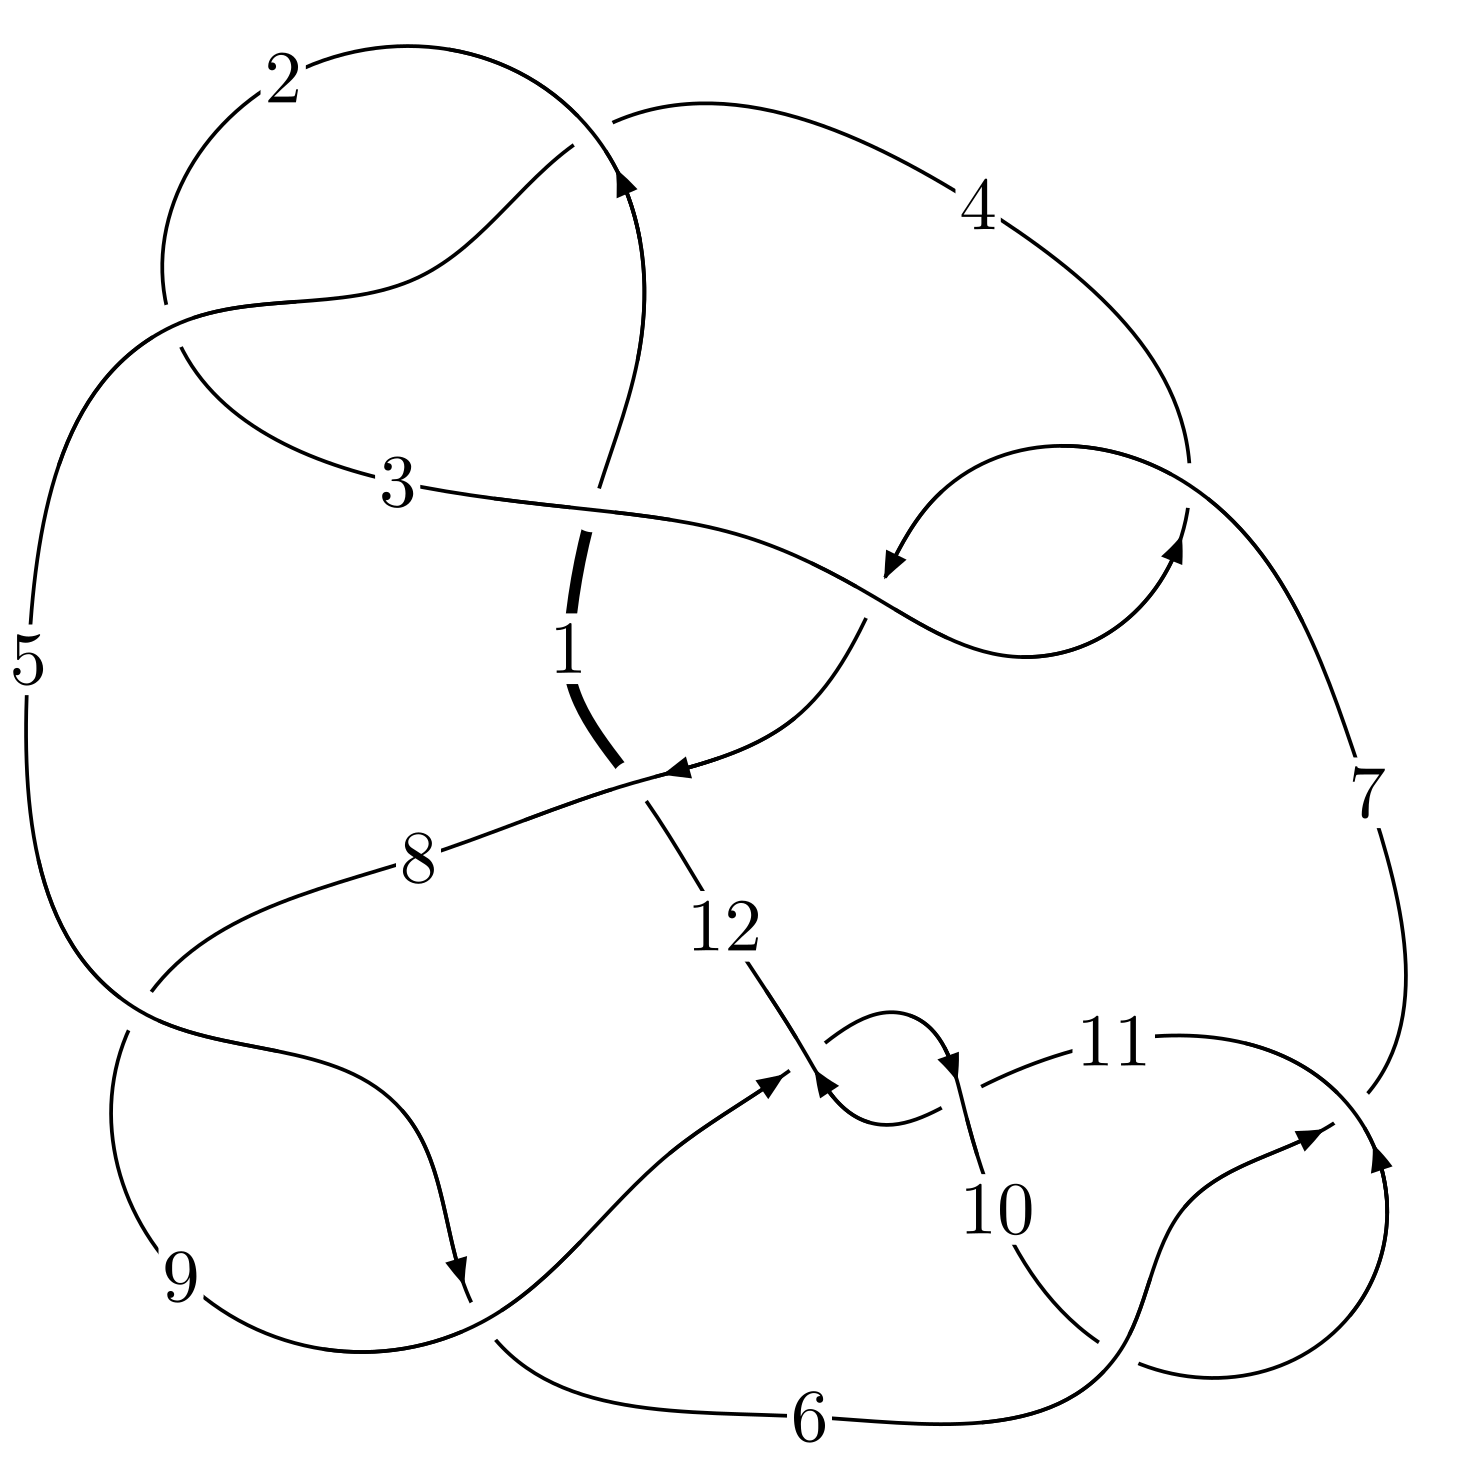
\includegraphics[width=112pt]{../../../GIT/diagram.site/Diagrams/png/2248_12n_0159.png}\\
\ \ \ A knot diagram\footnotemark}&
\allowdisplaybreaks
\textbf{Linearized knot diagam} \\
\cline{2-2}
 &
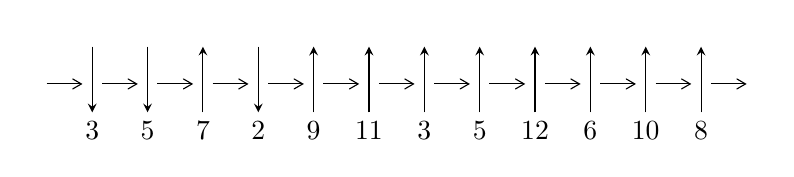
\begin{tikzpicture}[x=20pt, y=17pt]
	% nodes
	\node (C0) at (0, 0) {};
	\node (C1) at (1, 0) {};
	\node (C1U) at (1, +1) {};
	\node (C1D) at (1, -1) {3};

	\node (C2) at (2, 0) {};
	\node (C2U) at (2, +1) {};
	\node (C2D) at (2, -1) {5};

	\node (C3) at (3, 0) {};
	\node (C3U) at (3, +1) {};
	\node (C3D) at (3, -1) {7};

	\node (C4) at (4, 0) {};
	\node (C4U) at (4, +1) {};
	\node (C4D) at (4, -1) {2};

	\node (C5) at (5, 0) {};
	\node (C5U) at (5, +1) {};
	\node (C5D) at (5, -1) {9};

	\node (C6) at (6, 0) {};
	\node (C6U) at (6, +1) {};
	\node (C6D) at (6, -1) {11};

	\node (C7) at (7, 0) {};
	\node (C7U) at (7, +1) {};
	\node (C7D) at (7, -1) {3};

	\node (C8) at (8, 0) {};
	\node (C8U) at (8, +1) {};
	\node (C8D) at (8, -1) {5};

	\node (C9) at (9, 0) {};
	\node (C9U) at (9, +1) {};
	\node (C9D) at (9, -1) {12};

	\node (C10) at (10, 0) {};
	\node (C10U) at (10, +1) {};
	\node (C10D) at (10, -1) {6};

	\node (C11) at (11, 0) {};
	\node (C11U) at (11, +1) {};
	\node (C11D) at (11, -1) {10};

	\node (C12) at (12, 0) {};
	\node (C12U) at (12, +1) {};
	\node (C12D) at (12, -1) {8};
	\node (C13) at (13, 0) {};

	% arrows
	\draw[->,>={angle 60}]
	(C0) edge (C1) (C1) edge (C2) (C2) edge (C3) (C3) edge (C4) (C4) edge (C5) (C5) edge (C6) (C6) edge (C7) (C7) edge (C8) (C8) edge (C9) (C9) edge (C10) (C10) edge (C11) (C11) edge (C12) (C12) edge (C13) ;	\draw[->,>=stealth]
	(C1U) edge (C1D) (C2U) edge (C2D) (C3D) edge (C3U) (C4U) edge (C4D) (C5D) edge (C5U) (C6D) edge (C6U) (C7D) edge (C7U) (C8D) edge (C8U) (C9D) edge (C9U) (C10D) edge (C10U) (C11D) edge (C11U) (C12D) edge (C12U) ;
	\end{tikzpicture} \\
\hhline{~~} \\& 
\textbf{Solving Sequence} \\ \cline{2-2} 
 &
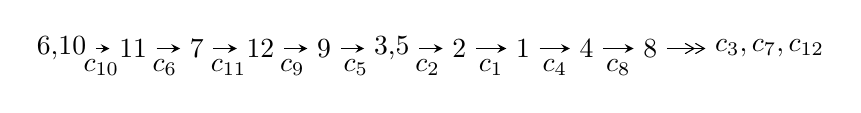
\begin{tikzpicture}[x=23pt, y=7pt]
	% node
	\node (A0) at (-1/8, 0) {6,10};
	\node (A1) at (1, 0) {11};
	\node (A2) at (2, 0) {7};
	\node (A3) at (3, 0) {12};
	\node (A4) at (4, 0) {9};
	\node (A5) at (81/16, 0) {3,5};
	\node (A6) at (49/8, 0) {2};
	\node (A7) at (57/8, 0) {1};
	\node (A8) at (65/8, 0) {4};
	\node (A9) at (73/8, 0) {8};
	\node (C1) at (1/2, -1) {$c_{10}$};
	\node (C2) at (3/2, -1) {$c_{6}$};
	\node (C3) at (5/2, -1) {$c_{11}$};
	\node (C4) at (7/2, -1) {$c_{9}$};
	\node (C5) at (9/2, -1) {$c_{5}$};
	\node (C6) at (45/8, -1) {$c_{2}$};
	\node (C7) at (53/8, -1) {$c_{1}$};
	\node (C8) at (61/8, -1) {$c_{4}$};
	\node (C9) at (69/8, -1) {$c_{8}$};
	\node (A10) at (11, 0) {$c_{3},c_{7},c_{12}$};

	% edge
	\draw[->,>=stealth]	
	(A0) edge (A1) (A1) edge (A2) (A2) edge (A3) (A3) edge (A4) (A4) edge (A5) (A5) edge (A6) (A6) edge (A7) (A7) edge (A8) (A8) edge (A9) ;
	\draw[->>,>={angle 60}]	
	(A9) edge (A10);
\end{tikzpicture} \\ 

\end{tabular} \\

\footnotetext{
The image of knot diagram is generated by the software ``\textbf{Draw programme}" developed by Andrew Bartholomew(\url{http://www.layer8.co.uk/maths/draw/index.htm\#Running-draw}), where we modified some parts for our purpose(\url{https://github.com/CATsTAILs/LinksPainter}).
}\phantom \\ \newline 
\centering \textbf{Ideals for irreducible components\footnotemark of $X_{\text{par}}$} 
 
\begin{align*}
I^u_{1}&=\langle 
u^{34}+2 u^{33}+\cdots+b-1,\;- u^{34}+5 u^{32}+\cdots+a+3 u,\;u^{35}+2 u^{34}+\cdots-2 u-1\rangle \\
I^u_{2}&=\langle 
- u^5+u^3- u^2+b- u,\;- u^7+u^5- u^4- u^3+a-1,\;u^8- u^7- u^6+2 u^5+u^4-2 u^3+2 u-1\rangle \\
\\
\end{align*}
\raggedright * 2 irreducible components of $\dim_{\mathbb{C}}=0$, with total 43 representations.\\
\footnotetext{All coefficients of polynomials are rational numbers. But the coefficients are sometimes approximated in decimal forms when there is not enough margin.}
\newpage
\renewcommand{\arraystretch}{1}
\centering \section*{I. $I^u_{1}= \langle u^{34}+2 u^{33}+\cdots+b-1,\;- u^{34}+5 u^{32}+\cdots+a+3 u,\;u^{35}+2 u^{34}+\cdots-2 u-1 \rangle$}
\flushleft \textbf{(i) Arc colorings}\\
\begin{tabular}{m{7pt} m{180pt} m{7pt} m{180pt} }
\flushright $a_{6}=$&$\begin{pmatrix}0\\u\end{pmatrix}$ \\
\flushright $a_{10}=$&$\begin{pmatrix}1\\0\end{pmatrix}$ \\
\flushright $a_{11}=$&$\begin{pmatrix}1\\- u^2\end{pmatrix}$ \\
\flushright $a_{7}=$&$\begin{pmatrix}u\\- u^3+u\end{pmatrix}$ \\
\flushright $a_{12}=$&$\begin{pmatrix}- u^2+1\\- u^2\end{pmatrix}$ \\
\flushright $a_{9}=$&$\begin{pmatrix}u^4- u^2+1\\u^4\end{pmatrix}$ \\
\flushright $a_{3}=$&$\begin{pmatrix}u^{34}-5 u^{32}+\cdots+3 u^2-3 u\\- u^{34}-2 u^{33}+\cdots+2 u+1\end{pmatrix}$ \\
\flushright $a_{5}=$&$\begin{pmatrix}- u^9+2 u^7-3 u^5+2 u^3- u\\- u^9+u^7- u^5+u\end{pmatrix}$ \\
\flushright $a_{2}=$&$\begin{pmatrix}u^{34}+u^{33}+\cdots-3 u-1\\- u^{29}+5 u^{27}+\cdots- u^3+3 u^2\end{pmatrix}$ \\
\flushright $a_{1}=$&$\begin{pmatrix}u^{26}-5 u^{24}+\cdots+3 u^2-1\\u^{26}-4 u^{24}+\cdots+2 u^4+u^2\end{pmatrix}$ \\
\flushright $a_{4}=$&$\begin{pmatrix}u^{34}+u^{33}+\cdots-4 u-1\\u^{34}+u^{33}+\cdots- u-1\end{pmatrix}$ \\
\flushright $a_{8}=$&$\begin{pmatrix}- u^{14}+3 u^{12}-6 u^{10}+7 u^8-6 u^6+4 u^4-2 u^2+1\\- u^{14}+2 u^{12}-3 u^{10}+2 u^8+u^2\end{pmatrix}$\\&\end{tabular}
\flushleft \textbf{(ii) Obstruction class $= -1$}\\~\\
\flushleft \textbf{(iii) Cusp Shapes $= -7 u^{34}-6 u^{33}+39 u^{32}+43 u^{31}-141 u^{30}-173 u^{29}+355 u^{28}+506 u^{27}-686 u^{26}-1134 u^{25}+1034 u^{24}+2071 u^{23}-1204 u^{22}-3115 u^{21}+1010 u^{20}+3917 u^{19}-424 u^{18}-4134 u^{17}-365 u^{16}+3614 u^{15}+1028 u^{14}-2600 u^{13}-1314 u^{12}+1451 u^{11}+1204 u^{10}-562 u^9-821 u^8+77 u^7+436 u^6+85 u^5-158 u^4-75 u^3+20 u^2+26 u+9$}\\~\\
\newpage\renewcommand{\arraystretch}{1}
\flushleft \textbf{(iv) u-Polynomials at the component}\newline \\
\begin{tabular}{m{50pt}|m{274pt}}
Crossings & \hspace{64pt}u-Polynomials at each crossing \\
\hline $$\begin{aligned}c_{1}\end{aligned}$$&$\begin{aligned}
&u^{35}+49 u^{34}+\cdots+102 u+1
\end{aligned}$\\
\hline $$\begin{aligned}c_{2},c_{4}\end{aligned}$$&$\begin{aligned}
&u^{35}-9 u^{34}+\cdots-14 u+1
\end{aligned}$\\
\hline $$\begin{aligned}c_{3},c_{7}\end{aligned}$$&$\begin{aligned}
&u^{35}- u^{34}+\cdots-640 u+256
\end{aligned}$\\
\hline $$\begin{aligned}c_{5},c_{8}\end{aligned}$$&$\begin{aligned}
&u^{35}-2 u^{34}+\cdots+108 u-36
\end{aligned}$\\
\hline $$\begin{aligned}c_{6},c_{10}\end{aligned}$$&$\begin{aligned}
&u^{35}+2 u^{34}+\cdots-2 u-1
\end{aligned}$\\
\hline $$\begin{aligned}c_{9},c_{11}\end{aligned}$$&$\begin{aligned}
&u^{35}-12 u^{34}+\cdots+2 u-1
\end{aligned}$\\
\hline $$\begin{aligned}c_{12}\end{aligned}$$&$\begin{aligned}
&u^{35}+36 u^{33}+\cdots-4 u+1
\end{aligned}$\\
\hline
\end{tabular}\\~\\
\newpage\renewcommand{\arraystretch}{1}
\flushleft \textbf{(v) Riley Polynomials at the component}\newline \\
\begin{tabular}{m{50pt}|m{274pt}}
Crossings & \hspace{64pt}Riley Polynomials at each crossing \\
\hline $$\begin{aligned}c_{1}\end{aligned}$$&$\begin{aligned}
&y^{35}-117 y^{34}+\cdots+6150 y-1
\end{aligned}$\\
\hline $$\begin{aligned}c_{2},c_{4}\end{aligned}$$&$\begin{aligned}
&y^{35}-49 y^{34}+\cdots+102 y-1
\end{aligned}$\\
\hline $$\begin{aligned}c_{3},c_{7}\end{aligned}$$&$\begin{aligned}
&y^{35}+51 y^{34}+\cdots+835584 y-65536
\end{aligned}$\\
\hline $$\begin{aligned}c_{5},c_{8}\end{aligned}$$&$\begin{aligned}
&y^{35}-12 y^{34}+\cdots+6840 y-1296
\end{aligned}$\\
\hline $$\begin{aligned}c_{6},c_{10}\end{aligned}$$&$\begin{aligned}
&y^{35}-12 y^{34}+\cdots+2 y-1
\end{aligned}$\\
\hline $$\begin{aligned}c_{9},c_{11}\end{aligned}$$&$\begin{aligned}
&y^{35}+24 y^{34}+\cdots+2 y-1
\end{aligned}$\\
\hline $$\begin{aligned}c_{12}\end{aligned}$$&$\begin{aligned}
&y^{35}+72 y^{34}+\cdots+2 y-1
\end{aligned}$\\
\hline
\end{tabular}\\~\\
\newpage\flushleft \textbf{(vi) Complex Volumes and Cusp Shapes}
$$\begin{array}{c|c|c}  
\text{Solutions to }I^u_{1}& \I (\text{vol} + \sqrt{-1}CS) & \text{Cusp shape}\\
 \hline 
\begin{aligned}
u &= \phantom{-}1.003180 + 0.076770 I \\
a &= -0.427602 + 0.732202 I \\
b &= \phantom{-}0.040765 - 1.055450 I\end{aligned}
 & \phantom{-}1.87836 + 2.29361 I & \phantom{-}9.35864 - 3.99437 I \\ \hline\begin{aligned}
u &= \phantom{-}1.003180 - 0.076770 I \\
a &= -0.427602 - 0.732202 I \\
b &= \phantom{-}0.040765 + 1.055450 I\end{aligned}
 & \phantom{-}1.87836 - 2.29361 I & \phantom{-}9.35864 + 3.99437 I \\ \hline\begin{aligned}
u &= -0.792898 + 0.645336 I \\
a &= -0.232938 - 0.928895 I \\
b &= \phantom{-}0.112888 - 0.720959 I\end{aligned}
 & -1.72435 - 2.14542 I & \phantom{-}5.01876 + 4.63119 I \\ \hline\begin{aligned}
u &= -0.792898 - 0.645336 I \\
a &= -0.232938 + 0.928895 I \\
b &= \phantom{-}0.112888 + 0.720959 I\end{aligned}
 & -1.72435 + 2.14542 I & \phantom{-}5.01876 - 4.63119 I \\ \hline\begin{aligned}
u &= -0.698567 + 0.764106 I \\
a &= \phantom{-}0.18575 + 2.20654 I \\
b &= -1.02864 + 2.02071 I\end{aligned}
 & -3.83985 + 2.10941 I & \phantom{-}1.06203 - 1.84479 I \\ \hline\begin{aligned}
u &= -0.698567 - 0.764106 I \\
a &= \phantom{-}0.18575 - 2.20654 I \\
b &= -1.02864 - 2.02071 I\end{aligned}
 & -3.83985 - 2.10941 I & \phantom{-}1.06203 + 1.84479 I \\ \hline\begin{aligned}
u &= \phantom{-}0.753011 + 0.738009 I \\
a &= \phantom{-}1.37904 - 1.86948 I \\
b &= -0.93662 - 2.24841 I\end{aligned}
 & -4.73261 + 0.86629 I & \phantom{-}0.579778 - 0.147183 I \\ \hline\begin{aligned}
u &= \phantom{-}0.753011 - 0.738009 I \\
a &= \phantom{-}1.37904 + 1.86948 I \\
b &= -0.93662 + 2.24841 I\end{aligned}
 & -4.73261 - 0.86629 I & \phantom{-}0.579778 + 0.147183 I \\ \hline\begin{aligned}
u &= -0.650584 + 0.839948 I \\
a &= -0.26514 - 2.94245 I \\
b &= \phantom{-}1.70386 - 2.51843 I\end{aligned}
 & -13.3967 + 6.2863 I & \phantom{-}1.00799 - 1.99078 I \\ \hline\begin{aligned}
u &= -0.650584 - 0.839948 I \\
a &= -0.26514 + 2.94245 I \\
b &= \phantom{-}1.70386 + 2.51843 I\end{aligned}
 & -13.3967 - 6.2863 I & \phantom{-}1.00799 + 1.99078 I\\
 \hline 
 \end{array}$$\newpage$$\begin{array}{c|c|c}  
\text{Solutions to }I^u_{1}& \I (\text{vol} + \sqrt{-1}CS) & \text{Cusp shape}\\
 \hline 
\begin{aligned}
u &= \phantom{-}0.597910 + 0.716545 I \\
a &= -0.474108 + 0.553918 I \\
b &= \phantom{-}0.273509 + 0.526339 I\end{aligned}
 & \phantom{-}0.466250 - 0.951396 I & \phantom{-}10.00295 + 0.38249 I \\ \hline\begin{aligned}
u &= \phantom{-}0.597910 - 0.716545 I \\
a &= -0.474108 - 0.553918 I \\
b &= \phantom{-}0.273509 - 0.526339 I\end{aligned}
 & \phantom{-}0.466250 + 0.951396 I & \phantom{-}10.00295 - 0.38249 I \\ \hline\begin{aligned}
u &= -0.922847\phantom{ +0.000000I} \\
a &= -1.31041\phantom{ +0.000000I} \\
b &= -1.21035\phantom{ +0.000000I}\end{aligned}
 & \phantom{-}0.182011\phantom{ +0.000000I} & \phantom{-}10.8590\phantom{ +0.000000I} \\ \hline\begin{aligned}
u &= -1.08201\phantom{ +0.000000I} \\
a &= \phantom{-}0.437613\phantom{ +0.000000I} \\
b &= \phantom{-}0.472974\phantom{ +0.000000I}\end{aligned}
 & \phantom{-}5.82108\phantom{ +0.000000I} & \phantom{-}17.0620\phantom{ +0.000000I} \\ \hline\begin{aligned}
u &= \phantom{-}1.111560 + 0.128216 I \\
a &= \phantom{-}1.138050 - 0.133066 I \\
b &= \phantom{-}0.300334 + 1.303030 I\end{aligned}
 & -6.72567 + 5.75996 I & \phantom{-}7.32314 - 3.54445 I \\ \hline\begin{aligned}
u &= \phantom{-}1.111560 - 0.128216 I \\
a &= \phantom{-}1.138050 + 0.133066 I \\
b &= \phantom{-}0.300334 - 1.303030 I\end{aligned}
 & -6.72567 - 5.75996 I & \phantom{-}7.32314 + 3.54445 I \\ \hline\begin{aligned}
u &= -0.934946 + 0.641378 I \\
a &= -0.922641 - 0.641680 I \\
b &= \phantom{-}0.090797 - 0.681520 I\end{aligned}
 & -1.26680 - 2.86899 I & \phantom{-}5.76020 + 1.94310 I \\ \hline\begin{aligned}
u &= -0.934946 - 0.641378 I \\
a &= -0.922641 + 0.641680 I \\
b &= \phantom{-}0.090797 + 0.681520 I\end{aligned}
 & -1.26680 + 2.86899 I & \phantom{-}5.76020 - 1.94310 I \\ \hline\begin{aligned}
u &= -1.036700 + 0.513296 I \\
a &= \phantom{-}0.468566 + 0.238758 I \\
b &= \phantom{-}0.355938 - 0.949026 I\end{aligned}
 & -9.06115 - 1.11837 I & \phantom{-}4.93303 + 2.48933 I \\ \hline\begin{aligned}
u &= -1.036700 - 0.513296 I \\
a &= \phantom{-}0.468566 - 0.238758 I \\
b &= \phantom{-}0.355938 + 0.949026 I\end{aligned}
 & -9.06115 + 1.11837 I & \phantom{-}4.93303 - 2.48933 I\\
 \hline 
 \end{array}$$\newpage$$\begin{array}{c|c|c}  
\text{Solutions to }I^u_{1}& \I (\text{vol} + \sqrt{-1}CS) & \text{Cusp shape}\\
 \hline 
\begin{aligned}
u &= \phantom{-}0.958291 + 0.699514 I \\
a &= \phantom{-}1.42433 - 1.41318 I \\
b &= -0.04365 - 2.87306 I\end{aligned}
 & -4.10408 + 4.62202 I & \phantom{-}2.53243 - 5.37025 I \\ \hline\begin{aligned}
u &= \phantom{-}0.958291 - 0.699514 I \\
a &= \phantom{-}1.42433 + 1.41318 I \\
b &= -0.04365 + 2.87306 I\end{aligned}
 & -4.10408 - 4.62202 I & \phantom{-}2.53243 + 5.37025 I \\ \hline\begin{aligned}
u &= \phantom{-}0.878474 + 0.799434 I \\
a &= -2.09357 + 2.58300 I \\
b &= \phantom{-}0.51980 + 3.81456 I\end{aligned}
 & -17.4916 + 2.9871 I & -0.26712 - 2.67515 I \\ \hline\begin{aligned}
u &= \phantom{-}0.878474 - 0.799434 I \\
a &= -2.09357 - 2.58300 I \\
b &= \phantom{-}0.51980 - 3.81456 I\end{aligned}
 & -17.4916 - 2.9871 I & -0.26712 + 2.67515 I \\ \hline\begin{aligned}
u &= \phantom{-}1.021530 + 0.658784 I \\
a &= -0.388047 + 0.431455 I \\
b &= -0.012993 + 0.931220 I\end{aligned}
 & \phantom{-}1.70279 + 6.25040 I & \phantom{-}12.13050 - 4.97456 I \\ \hline\begin{aligned}
u &= \phantom{-}1.021530 - 0.658784 I \\
a &= -0.388047 - 0.431455 I \\
b &= -0.012993 - 0.931220 I\end{aligned}
 & \phantom{-}1.70279 - 6.25040 I & \phantom{-}12.13050 + 4.97456 I \\ \hline\begin{aligned}
u &= -0.993451 + 0.702180 I \\
a &= \phantom{-}2.14762 + 0.79394 I \\
b &= \phantom{-}0.45485 + 2.36980 I\end{aligned}
 & -2.94898 - 7.68050 I & \phantom{-}3.12136 + 6.96771 I \\ \hline\begin{aligned}
u &= -0.993451 - 0.702180 I \\
a &= \phantom{-}2.14762 - 0.79394 I \\
b &= \phantom{-}0.45485 - 2.36980 I\end{aligned}
 & -2.94898 + 7.68050 I & \phantom{-}3.12136 - 6.96771 I \\ \hline\begin{aligned}
u &= -0.263163 + 0.716876 I \\
a &= -1.150580 + 0.479086 I \\
b &= \phantom{-}0.686293 - 0.231426 I\end{aligned}
 & -11.29280 - 3.30354 I & \phantom{-}1.02998 + 2.25929 I \\ \hline\begin{aligned}
u &= -0.263163 - 0.716876 I \\
a &= -1.150580 - 0.479086 I \\
b &= \phantom{-}0.686293 + 0.231426 I\end{aligned}
 & -11.29280 + 3.30354 I & \phantom{-}1.02998 - 2.25929 I\\
 \hline 
 \end{array}$$\newpage$$\begin{array}{c|c|c}  
\text{Solutions to }I^u_{1}& \I (\text{vol} + \sqrt{-1}CS) & \text{Cusp shape}\\
 \hline 
\begin{aligned}
u &= -1.039590 + 0.718934 I \\
a &= -2.70067 - 0.80992 I \\
b &= -1.22822 - 3.37949 I\end{aligned}
 & -12.2131 - 12.1134 I & \phantom{-}2.82361 + 6.65221 I \\ \hline\begin{aligned}
u &= -1.039590 - 0.718934 I \\
a &= -2.70067 + 0.80992 I \\
b &= -1.22822 + 3.37949 I\end{aligned}
 & -12.2131 + 12.1134 I & \phantom{-}2.82361 - 6.65221 I \\ \hline\begin{aligned}
u &= \phantom{-}0.515516\phantom{ +0.000000I} \\
a &= -0.450972\phantom{ +0.000000I} \\
b &= \phantom{-}0.317465\phantom{ +0.000000I}\end{aligned}
 & \phantom{-}0.694754\phantom{ +0.000000I} & \phantom{-}14.6380\phantom{ +0.000000I} \\ \hline\begin{aligned}
u &= -0.169379 + 0.388841 I \\
a &= \phantom{-}0.57383 - 1.55781 I \\
b &= -0.578952 - 0.351526 I\end{aligned}
 & -1.66775 - 0.90576 I & -1.19698 + 2.88649 I \\ \hline\begin{aligned}
u &= -0.169379 - 0.388841 I \\
a &= \phantom{-}0.57383 + 1.55781 I \\
b &= -0.578952 + 0.351526 I\end{aligned}
 & -1.66775 + 0.90576 I & -1.19698 - 2.88649 I\\
 \hline 
 \end{array}$$\newpage\newpage\renewcommand{\arraystretch}{1}
\centering \section*{II. $I^u_{2}= \langle - u^5+u^3- u^2+b- u,\;- u^7+u^5- u^4- u^3+a-1,\;u^8- u^7- u^6+2 u^5+u^4-2 u^3+2 u-1 \rangle$}
\flushleft \textbf{(i) Arc colorings}\\
\begin{tabular}{m{7pt} m{180pt} m{7pt} m{180pt} }
\flushright $a_{6}=$&$\begin{pmatrix}0\\u\end{pmatrix}$ \\
\flushright $a_{10}=$&$\begin{pmatrix}1\\0\end{pmatrix}$ \\
\flushright $a_{11}=$&$\begin{pmatrix}1\\- u^2\end{pmatrix}$ \\
\flushright $a_{7}=$&$\begin{pmatrix}u\\- u^3+u\end{pmatrix}$ \\
\flushright $a_{12}=$&$\begin{pmatrix}- u^2+1\\- u^2\end{pmatrix}$ \\
\flushright $a_{9}=$&$\begin{pmatrix}u^4- u^2+1\\u^4\end{pmatrix}$ \\
\flushright $a_{3}=$&$\begin{pmatrix}u^7- u^5+u^4+u^3+1\\u^5- u^3+u^2+u\end{pmatrix}$ \\
\flushright $a_{5}=$&$\begin{pmatrix}u^6- u^4+2 u^2-1\\- u^7+u^6+2 u^5- u^4-2 u^3+2 u^2+2 u-1\end{pmatrix}$ \\
\flushright $a_{2}=$&$\begin{pmatrix}u^7- u^6- u^5+2 u^4+u^3-2 u^2+2\\u^7- u^6- u^5+u^4+u^3- u^2- u+1\end{pmatrix}$ \\
\flushright $a_{1}=$&$\begin{pmatrix}- u^6+u^4-2 u^2+1\\u^7- u^6-2 u^5+u^4+2 u^3-2 u^2-2 u+1\end{pmatrix}$ \\
\flushright $a_{4}=$&$\begin{pmatrix}u^7- u^5+u^4+u^3+1\\u^5- u^3+u^2+u\end{pmatrix}$ \\
\flushright $a_{8}=$&$\begin{pmatrix}u\\- u^3+u\end{pmatrix}$\\&\end{tabular}
\flushleft \textbf{(ii) Obstruction class $= 1$}\\~\\
\flushleft \textbf{(iii) Cusp Shapes $= 2 u^7+u^6-5 u^5+5 u^3- u^2-4 u+5$}\\~\\
\newpage\renewcommand{\arraystretch}{1}
\flushleft \textbf{(iv) u-Polynomials at the component}\newline \\
\begin{tabular}{m{50pt}|m{274pt}}
Crossings & \hspace{64pt}u-Polynomials at each crossing \\
\hline $$\begin{aligned}c_{1},c_{2}\end{aligned}$$&$\begin{aligned}
&(u-1)^8
\end{aligned}$\\
\hline $$\begin{aligned}c_{3},c_{7}\end{aligned}$$&$\begin{aligned}
&u^8
\end{aligned}$\\
\hline $$\begin{aligned}c_{4}\end{aligned}$$&$\begin{aligned}
&(u+1)^8
\end{aligned}$\\
\hline $$\begin{aligned}c_{5}\end{aligned}$$&$\begin{aligned}
&u^8- u^7-3 u^6+2 u^5+3 u^4-2 u-1
\end{aligned}$\\
\hline $$\begin{aligned}c_{6}\end{aligned}$$&$\begin{aligned}
&u^8+u^7- u^6-2 u^5+u^4+2 u^3-2 u-1
\end{aligned}$\\
\hline $$\begin{aligned}c_{8},c_{12}\end{aligned}$$&$\begin{aligned}
&u^8+u^7-3 u^6-2 u^5+3 u^4+2 u-1
\end{aligned}$\\
\hline $$\begin{aligned}c_{9}\end{aligned}$$&$\begin{aligned}
&u^8+3 u^7+7 u^6+10 u^5+11 u^4+10 u^3+6 u^2+4 u+1
\end{aligned}$\\
\hline $$\begin{aligned}c_{10}\end{aligned}$$&$\begin{aligned}
&u^8- u^7- u^6+2 u^5+u^4-2 u^3+2 u-1
\end{aligned}$\\
\hline $$\begin{aligned}c_{11}\end{aligned}$$&$\begin{aligned}
&u^8-3 u^7+7 u^6-10 u^5+11 u^4-10 u^3+6 u^2-4 u+1
\end{aligned}$\\
\hline
\end{tabular}\\~\\
\newpage\renewcommand{\arraystretch}{1}
\flushleft \textbf{(v) Riley Polynomials at the component}\newline \\
\begin{tabular}{m{50pt}|m{274pt}}
Crossings & \hspace{64pt}Riley Polynomials at each crossing \\
\hline $$\begin{aligned}c_{1},c_{2},c_{4}\end{aligned}$$&$\begin{aligned}
&(y-1)^8
\end{aligned}$\\
\hline $$\begin{aligned}c_{3},c_{7}\end{aligned}$$&$\begin{aligned}
&y^8
\end{aligned}$\\
\hline $$\begin{aligned}c_{5},c_{8},c_{12}\end{aligned}$$&$\begin{aligned}
&y^8-7 y^7+19 y^6-22 y^5+3 y^4+14 y^3-6 y^2-4 y+1
\end{aligned}$\\
\hline $$\begin{aligned}c_{6},c_{10}\end{aligned}$$&$\begin{aligned}
&y^8-3 y^7+7 y^6-10 y^5+11 y^4-10 y^3+6 y^2-4 y+1
\end{aligned}$\\
\hline $$\begin{aligned}c_{9},c_{11}\end{aligned}$$&$\begin{aligned}
&y^8+5 y^7+11 y^6+6 y^5-17 y^4-34 y^3-22 y^2-4 y+1
\end{aligned}$\\
\hline
\end{tabular}\\~\\
\newpage\flushleft \textbf{(vi) Complex Volumes and Cusp Shapes}
$$\begin{array}{c|c|c}  
\text{Solutions to }I^u_{2}& \I (\text{vol} + \sqrt{-1}CS) & \text{Cusp shape}\\
 \hline 
\begin{aligned}
u &= \phantom{-}0.570868 + 0.730671 I \\
a &= \phantom{-}0.325934 + 0.693334 I \\
b &= \phantom{-}0.972127 + 0.565636 I\end{aligned}
 & -0.604279 - 1.131230 I & \phantom{-}1.47926 + 0.84929 I \\ \hline\begin{aligned}
u &= \phantom{-}0.570868 - 0.730671 I \\
a &= \phantom{-}0.325934 - 0.693334 I \\
b &= \phantom{-}0.972127 - 0.565636 I\end{aligned}
 & -0.604279 + 1.131230 I & \phantom{-}1.47926 - 0.84929 I \\ \hline\begin{aligned}
u &= -0.855237 + 0.665892 I \\
a &= -1.03462 - 0.99451 I \\
b &= \phantom{-}0.39611 - 1.88650 I\end{aligned}
 & -3.80435 - 2.57849 I & \phantom{-}2.50535 + 3.23297 I \\ \hline\begin{aligned}
u &= -0.855237 - 0.665892 I \\
a &= -1.03462 + 0.99451 I \\
b &= \phantom{-}0.39611 + 1.88650 I\end{aligned}
 & -3.80435 + 2.57849 I & \phantom{-}2.50535 - 3.23297 I \\ \hline\begin{aligned}
u &= -1.09818\phantom{ +0.000000I} \\
a &= \phantom{-}0.801005\phantom{ +0.000000I} \\
b &= -0.165005\phantom{ +0.000000I}\end{aligned}
 & \phantom{-}4.85780\phantom{ +0.000000I} & \phantom{-}7.45240\phantom{ +0.000000I} \\ \hline\begin{aligned}
u &= \phantom{-}1.031810 + 0.655470 I \\
a &= -0.842429 - 0.289836 I \\
b &= -0.699541 + 1.033710 I\end{aligned}
 & \phantom{-}0.73474 + 6.44354 I & \phantom{-}3.27544 - 5.90525 I \\ \hline\begin{aligned}
u &= \phantom{-}1.031810 - 0.655470 I \\
a &= -0.842429 + 0.289836 I \\
b &= -0.699541 - 1.033710 I\end{aligned}
 & \phantom{-}0.73474 - 6.44354 I & \phantom{-}3.27544 + 5.90525 I \\ \hline\begin{aligned}
u &= \phantom{-}0.603304\phantom{ +0.000000I} \\
a &= \phantom{-}1.30123\phantom{ +0.000000I} \\
b &= \phantom{-}0.827616\phantom{ +0.000000I}\end{aligned}
 & -0.799899\phantom{ +0.000000I} & \phantom{-}3.02750\phantom{ +0.000000I}\\
 \hline 
 \end{array}$$\newpage
\newpage\renewcommand{\arraystretch}{1}
\centering \section*{ III. u-Polynomials}
\begin{tabular}{m{50pt}|m{274pt}}
Crossings & \hspace{64pt}u-Polynomials at each crossing \\
\hline $$\begin{aligned}c_{1}\end{aligned}$$&$\begin{aligned}
&((u-1)^8)(u^{35}+49 u^{34}+\cdots+102 u+1)
\end{aligned}$\\
\hline $$\begin{aligned}c_{2}\end{aligned}$$&$\begin{aligned}
&((u-1)^8)(u^{35}-9 u^{34}+\cdots-14 u+1)
\end{aligned}$\\
\hline $$\begin{aligned}c_{3},c_{7}\end{aligned}$$&$\begin{aligned}
&u^8(u^{35}- u^{34}+\cdots-640 u+256)
\end{aligned}$\\
\hline $$\begin{aligned}c_{4}\end{aligned}$$&$\begin{aligned}
&((u+1)^8)(u^{35}-9 u^{34}+\cdots-14 u+1)
\end{aligned}$\\
\hline $$\begin{aligned}c_{5}\end{aligned}$$&$\begin{aligned}
&(u^8- u^7-3 u^6+2 u^5+3 u^4-2 u-1)(u^{35}-2 u^{34}+\cdots+108 u-36)
\end{aligned}$\\
\hline $$\begin{aligned}c_{6}\end{aligned}$$&$\begin{aligned}
&(u^8+u^7+\cdots-2 u-1)(u^{35}+2 u^{34}+\cdots-2 u-1)
\end{aligned}$\\
\hline $$\begin{aligned}c_{8}\end{aligned}$$&$\begin{aligned}
&(u^8+u^7-3 u^6-2 u^5+3 u^4+2 u-1)(u^{35}-2 u^{34}+\cdots+108 u-36)
\end{aligned}$\\
\hline $$\begin{aligned}c_{9}\end{aligned}$$&$\begin{aligned}
&(u^8+3 u^7+7 u^6+10 u^5+11 u^4+10 u^3+6 u^2+4 u+1)\\
&\cdot(u^{35}-12 u^{34}+\cdots+2 u-1)
\end{aligned}$\\
\hline $$\begin{aligned}c_{10}\end{aligned}$$&$\begin{aligned}
&(u^8- u^7+\cdots+2 u-1)(u^{35}+2 u^{34}+\cdots-2 u-1)
\end{aligned}$\\
\hline $$\begin{aligned}c_{11}\end{aligned}$$&$\begin{aligned}
&(u^8-3 u^7+7 u^6-10 u^5+11 u^4-10 u^3+6 u^2-4 u+1)\\
&\cdot(u^{35}-12 u^{34}+\cdots+2 u-1)
\end{aligned}$\\
\hline $$\begin{aligned}c_{12}\end{aligned}$$&$\begin{aligned}
&(u^8+u^7-3 u^6-2 u^5+3 u^4+2 u-1)(u^{35}+36 u^{33}+\cdots-4 u+1)
\end{aligned}$\\
\hline
\end{tabular}\newpage\renewcommand{\arraystretch}{1}
\centering \section*{ IV. Riley Polynomials}
\begin{tabular}{m{50pt}|m{274pt}}
Crossings & \hspace{64pt}Riley Polynomials at each crossing \\
\hline $$\begin{aligned}c_{1}\end{aligned}$$&$\begin{aligned}
&((y-1)^8)(y^{35}-117 y^{34}+\cdots+6150 y-1)
\end{aligned}$\\
\hline $$\begin{aligned}c_{2},c_{4}\end{aligned}$$&$\begin{aligned}
&((y-1)^8)(y^{35}-49 y^{34}+\cdots+102 y-1)
\end{aligned}$\\
\hline $$\begin{aligned}c_{3},c_{7}\end{aligned}$$&$\begin{aligned}
&y^8(y^{35}+51 y^{34}+\cdots+835584 y-65536)
\end{aligned}$\\
\hline $$\begin{aligned}c_{5},c_{8}\end{aligned}$$&$\begin{aligned}
&(y^8-7 y^7+19 y^6-22 y^5+3 y^4+14 y^3-6 y^2-4 y+1)\\
&\cdot(y^{35}-12 y^{34}+\cdots+6840 y-1296)
\end{aligned}$\\
\hline $$\begin{aligned}c_{6},c_{10}\end{aligned}$$&$\begin{aligned}
&(y^8-3 y^7+7 y^6-10 y^5+11 y^4-10 y^3+6 y^2-4 y+1)\\
&\cdot(y^{35}-12 y^{34}+\cdots+2 y-1)
\end{aligned}$\\
\hline $$\begin{aligned}c_{9},c_{11}\end{aligned}$$&$\begin{aligned}
&(y^8+5 y^7+11 y^6+6 y^5-17 y^4-34 y^3-22 y^2-4 y+1)\\
&\cdot(y^{35}+24 y^{34}+\cdots+2 y-1)
\end{aligned}$\\
\hline $$\begin{aligned}c_{12}\end{aligned}$$&$\begin{aligned}
&(y^8-7 y^7+19 y^6-22 y^5+3 y^4+14 y^3-6 y^2-4 y+1)\\
&\cdot(y^{35}+72 y^{34}+\cdots+2 y-1)
\end{aligned}$\\
\hline
\end{tabular}
\vskip 2pc
\end{document}